\documentclass[11pt]{article}

\usepackage[margin=1in]{geometry}
\usepackage{booktabs}
\usepackage{tikz}
\usepackage{listings}
\usepackage{xcolor}

\lstset{
	basicstyle=\ttfamily\footnotesize,
	frame=single,
	framesep=4pt,
	xleftmargin=6pt,
	breaklines=true,
	showstringspaces=false,
	language=C++
}

\title{Lab 2: Working with Processes \\ \large Operating Systems}
\author{Ayush Yadav (CS24BT001) \\ Trisham Bepari (CS24BT022) \\ IIT Dharwad}
\date{\today}

\begin{document}
\maketitle

\section*{Objective}
Search for a fixed pattern inside a large file, and use that as an excuse to learn
how processes are created with \texttt{fork}, replaced with \texttt{exec}, reaped
with \texttt{wait}, and terminated with \texttt{kill}. The work is split across
three parts: a single process doing the whole search, a tree of processes each
searching one chunk, and finally the same tree but with the useless work cancelled
as soon as the answer is known.

The input file \texttt{file.txt} is 67108864 bytes (64 MiB) and the pattern is
\texttt{NGTNIJGK}. The maximum chunk size used throughout Parts II and III is
8388608 bytes (8 MiB).

\section*{Part I: Searching a Range of the File}

\subsection*{Approach}
\texttt{part1\_searcher.cpp} takes a file, a pattern, and a start and end position,
and looks for the pattern only inside that range. The file is opened in binary mode
with \texttt{ifstream}, \texttt{seekg} moves the read head to the start position,
and one \texttt{read} pulls the whole range into a heap buffer. The buffer is
allocated one byte longer than the range so that a terminating null can be written
at the end, which lets \texttt{strstr} do the actual matching.

The number of bytes actually read comes from \texttt{gcount}, not from the
requested length. This matters when the caller asks for a range that runs past the
end of the file: the null then lands at the real end of the data instead of past
it. The match position reported to the user is the offset returned by
\texttt{strstr} added back to the start position, so it is an absolute position in
the file and not an offset inside the chunk.

\subsection*{Result}
Running \texttt{make run-part1} searches the whole file:

\begin{verbatim}
$ ./part1.out file.txt NGTNIJGK 0 67108863
[30822] found at 64520807
\end{verbatim}

The pattern sits at byte 64520807, which is quite close to the end of the file.
That single fact ends up shaping everything that happens in Parts II and III, since
it means the last chunk is the one that succeeds and every other chunk is wasted
effort.

The program returns 1 when the pattern is found and 0 when it is not. This return
value is what Part III later uses to decide whether the search is over. One small
annoyance showed up here: \texttt{make} treats a non zero exit status as a failed
recipe, so \texttt{run-part1} and \texttt{run-part3} end with \texttt{|| true} in
the makefile. Without it a successful search looks like a broken build.

\section*{Part II: Splitting the Search Across a Process Tree}

\subsection*{How the partitioning works}
\texttt{part2\_partitioner.cpp} is given a range and a maximum chunk size. It first
announces its own range, then decides between two behaviours:

\begin{itemize}
	\item If the range is larger than the maximum chunk size, it halves the range,
	forks twice, and each child execs a fresh copy of the partitioner on one half.
	The parent then does nothing except wait for both children.
	\item If the range fits within the maximum chunk size, it forks once and the
	child execs the searcher on that range.
	\texttt{part2\_searcher.out} is the Part I code, unchanged.
\end{itemize}

The split point is computed as
\texttt{search\_start\_position + search\_size / 2}, so the left child gets
everything below it and the right child everything from it onward. The recursion
is driven entirely by \texttt{exec}, not by a recursive function call, which is why
\texttt{argv[0]} is reused as the program to exec: the partitioner relaunches
itself.

\begin{lstlisting}
int left_end_position = search_start_position + search_size / 2 - 1;

my_children[0] = fork();
if(my_children[0] == 0)
{
        execl(argv[0], argv[0], file_to_search_in, pattern_to_search_for,
              left_start.c_str(), left_end.c_str(), argv[5], (char *)NULL);
        return -1;
}
\end{lstlisting}

With a 64 MiB file and an 8 MiB chunk limit, the range halves three times before it
stops being larger than the limit. That gives 1 + 2 + 4 + 8 = 15 partitioner
processes and 8 searcher processes, so 23 processes in total. The counts in the
captured log agree: 15 lines reporting a start position, 7 lines reporting a left
child fork, and 8 lines reporting a searcher fork.

\subsection*{The process tree}

Figure~\ref{fig:tree} shows the tree. Solid boxes are partitioner processes and
dashed boxes are searcher processes. Ranges are written in MiB for readability; the
exact byte ranges of the eight leaf chunks are listed in Table~\ref{tab:chunks}.

\begin{figure}[h]
\centering
\resizebox{\textwidth}{!}{
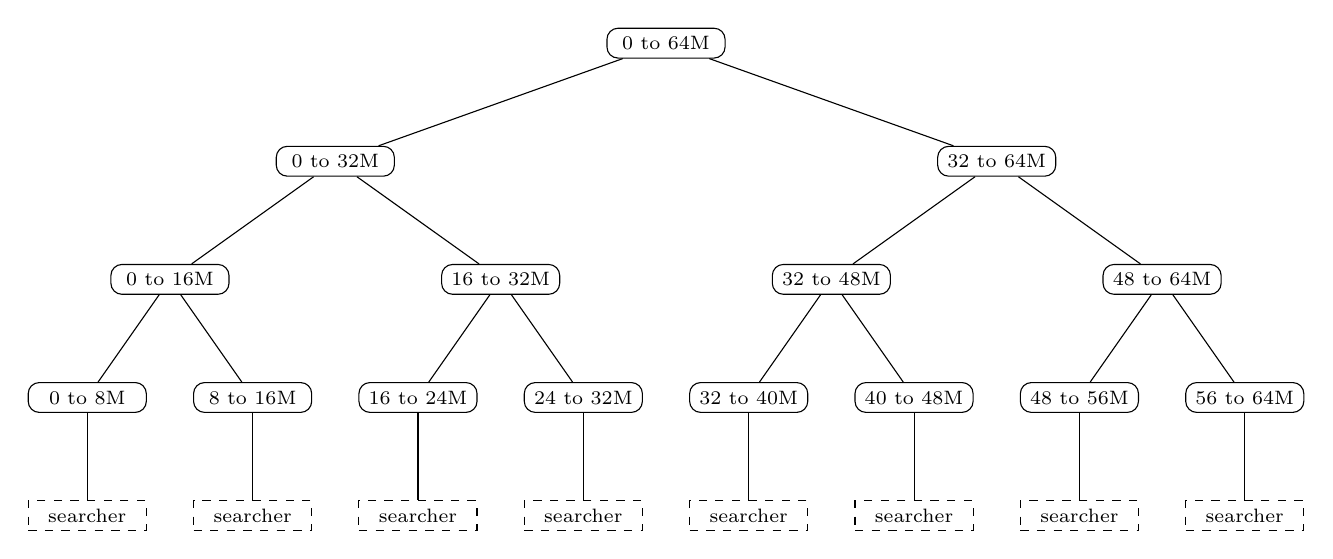
\begin{tikzpicture}[
	level distance=1.5cm,
	every node/.style={font=\scriptsize},
	part/.style={draw, rounded corners, inner sep=3pt, minimum width=1.5cm, align=center},
	search/.style={draw, dashed, inner sep=3pt, minimum width=1.5cm, align=center},
	level 1/.style={sibling distance=8.4cm},
	level 2/.style={sibling distance=4.2cm},
	level 3/.style={sibling distance=2.1cm},
	level 4/.style={sibling distance=2.1cm}
]
\node[part] {0 to 64M}
	child {node[part] {0 to 32M}
		child {node[part] {0 to 16M}
			child {node[part] {0 to 8M} child {node[search] {searcher}}}
			child {node[part] {8 to 16M} child {node[search] {searcher}}}
		}
		child {node[part] {16 to 32M}
			child {node[part] {16 to 24M} child {node[search] {searcher}}}
			child {node[part] {24 to 32M} child {node[search] {searcher}}}
		}
	}
	child {node[part] {32 to 64M}
		child {node[part] {32 to 48M}
			child {node[part] {32 to 40M} child {node[search] {searcher}}}
			child {node[part] {40 to 48M} child {node[search] {searcher}}}
		}
		child {node[part] {48 to 64M}
			child {node[part] {48 to 56M} child {node[search] {searcher}}}
			child {node[part] {56 to 64M} child {node[search] {searcher}}}
		}
	};
\end{tikzpicture}
}
\caption{Process tree for Part II. Every internal node is a partitioner that forked
two partitioners; every leaf partitioner forked one searcher. 15 partitioners and 8
searchers.}
\label{fig:tree}
\end{figure}

\begin{table}[h]
	\centering
	\begin{tabular}{crrl}
		\toprule
		Chunk & Start & End & Outcome \\
		\midrule
		1 & 0 & 8388607 & didn't find \\
		2 & 8388608 & 16777215 & didn't find \\
		3 & 16777216 & 25165823 & didn't find \\
		4 & 25165824 & 33554431 & didn't find \\
		5 & 33554432 & 41943039 & didn't find \\
		6 & 41943040 & 50331647 & didn't find \\
		7 & 50331648 & 58720255 & didn't find \\
		8 & 58720256 & 67108863 & found at 64520807 \\
		\bottomrule
	\end{tabular}
	\caption{The eight leaf chunks and what each searcher reported.}
	\label{tab:chunks}
\end{table}

\subsection*{Order in which processes were created}
Creation is strictly top down and breadth first by level, because a process cannot
fork a child until it has itself been forked and exec'd. Using the PIDs from the
captured run in Appendix A:

\begin{enumerate}
	\item \textbf{Level 0.} 30824 starts on 0 to 67108863.
	\item \textbf{Level 1.} 30824 forks 30825 (left, 0 to 33554431) and then 30826
	(right, 33554432 to 67108863).
	\item \textbf{Level 2.} 30825 forks 30827 and 30829; 30826 forks 30828 and
	30830. These four cover the 16 MiB ranges.
	\item \textbf{Level 3.} 30827 forks 30831 and 30834; 30829 forks 30833 and
	30836; 30828 forks 30832 and 30835; 30830 forks 30837 and 30838. These eight
	cover the 8 MiB ranges.
	\item \textbf{Searchers.} Each level 3 partitioner forks exactly one searcher:
	30842, 30841, 30840, 30844, 30839, 30843, 30845 and 30846.
\end{enumerate}

Within a level the interleaving is not fixed. In the captured log 30826 prints its
start position before 30825 does, even though 30825 was forked first, and the
searcher PIDs are not handed out in left to right order. Once two processes exist
the scheduler decides who runs next, so only the parent to child ordering is
guaranteed.

\subsection*{Order in which processes terminated}
Termination runs in the opposite direction, bottom up, and for a structural reason:
a partitioner blocks in \texttt{wait} until its children are gone, so no parent can
exit before its subtree has. The observed order was:

\begin{enumerate}
	\item The eight searchers exit first, in whatever order they finish reading
	their chunk. 30846 was the one that found the pattern, and it happened to
	finish before the other seven.
	\item Each leaf partitioner exits as soon as its own searcher is reaped, and it prints
	\texttt{searcher child returned}.
	\item The four level 2 partitioners exit once both of their children are reaped,
	then the two level 1 partitioners, and finally the root 30824.
\end{enumerate}

The parent does not choose the order in which it reaps. \texttt{wait} is called
without a PID and returns whichever child died first, and the returned PID is
compared against the stored left and right child PIDs to decide which message to
print. That is why the log contains \texttt{right child returned} before
\texttt{left child returned} for 30826, 30829 and 30825: their right subtree simply
finished first.

\begin{lstlisting}
for(int i = 0; i < 2; i++)
{
        pid_t finished_child = wait(NULL);
        if(finished_child == my_children[0])
                cout << "[" << my_pid << "] left child returned\n";
        else
                cout << "[" << my_pid << "] right child returned\n";
        cout.flush();
}
\end{lstlisting}

The obvious waste is visible in the log: 30846 reports the match very early, and
the other seven searchers keep scanning their 8 MiB chunks anyway. Part III fixes
this.

\section*{Part III: Cancelling the Search Once the Pattern Is Found}

\subsection*{Design}
Two things need to happen once a searcher succeeds. The good news has to travel up
the tree, and the kill order has to travel back down every other branch.

Upward travel reuses the exit status. The searcher already returns 1 on success, so
a partitioner inspects the status from \texttt{wait} with \texttt{WIFEXITED} and
\texttt{WEXITSTATUS} and sets its own return value to 1 if a child reported 1. The
status therefore climbs one level per reaped child until it reaches the root.

Downward travel uses \texttt{SIGTERM}. A partitioner that learns the pattern was
found stops waiting for its other child, sends it \texttt{SIGTERM}, and reaps it.
Every partitioner installs a handler for \texttt{SIGTERM} that prints the message,
forwards the same signal to whichever of its own children are still alive, and
exits. Because each process only ever signals its own direct children, the kill
travels down the doomed subtree one level at a time on its own.

\begin{lstlisting}
pid_t my_children[2] = {0, 0};

void handle_sigterm(int signal_number)
{
        cout << "[" << getpid() << "] received SIGTERM\n";
        cout.flush();
        for(int i = 0; i < 2; i++)
                if(my_children[i] > 0)
                        kill(my_children[i], SIGTERM);
        _exit(0);
}
\end{lstlisting}

The children array is a global because a signal handler cannot be handed
parameters. Entries are set to 0 as soon as a child is reaped, so the handler never
signals a PID that has already been recycled by the kernel. The searcher gets a
handler too, a simpler one that just prints and exits, since a searcher that is
midway through a chunk should also stop.

\texttt{\_exit} is used instead of \texttt{exit} inside the handler. \texttt{exit}
would flush the C++ stream buffers a second time from inside a signal context, and
the explicit \texttt{cout.flush()} already took care of the output.

\subsection*{Order in which processes were created and killed}
Creation is identical to Part II, since nothing about the partitioning changed. The
interesting part is the shutdown. Using the run in Appendix B, where 31116 is the
root and 31138 is the searcher on the last chunk:

\begin{enumerate}
	\item 31138 prints \texttt{found at 64520807} and exits with status 1.
	\item Its parent 31130 (56 to 64M) reaps it, prints \texttt{searcher child
	returned}, and exits with status 1.
	\item 31122 (48 to 64M) reaps 31130 as its right child, sees status 1, and
	sends \texttt{SIGTERM} to its left child 31128. 31128 prints its message and
	forwards the signal to its own searcher 31134. Both die.
	\item 31122 exits with status 1. 31118 (32 to 64M) reaps it, sees status 1, and
	kills its left child 31121. 31121 forwards to 31129, which forwards to its
	searcher 31137.
	\item 31118 exits with status 1. The root 31116 reaps it, sees status 1, and
	kills its left child 31117, which is the entire first half of the file. The
	signal walks down through 31120, then 31125 and 31126, then their searchers
	31133 and 31136.
	\item The root exits with status 1 and the run is over.
\end{enumerate}

So the kill order is: 31128 and 31134, then 31121, 31129 and 31137, then 31117,
31120, 31125, 31126, 31133 and 31136. Eleven processes were terminated in this run
instead of being allowed to finish. Notice that the killing goes strictly right to
left up the tree, which is exactly what we would expect given that the match is in
the very last chunk. The three kills correspond to the three left siblings on the
path from the winning leaf back to the root.

Figure~\ref{fig:kill} marks the same tree. The path from the winning chunk to the
root carries the status upward, and each shaded subtree is a whole branch that got
signalled.

\begin{figure}[h]
\centering
\resizebox{\textwidth}{!}{
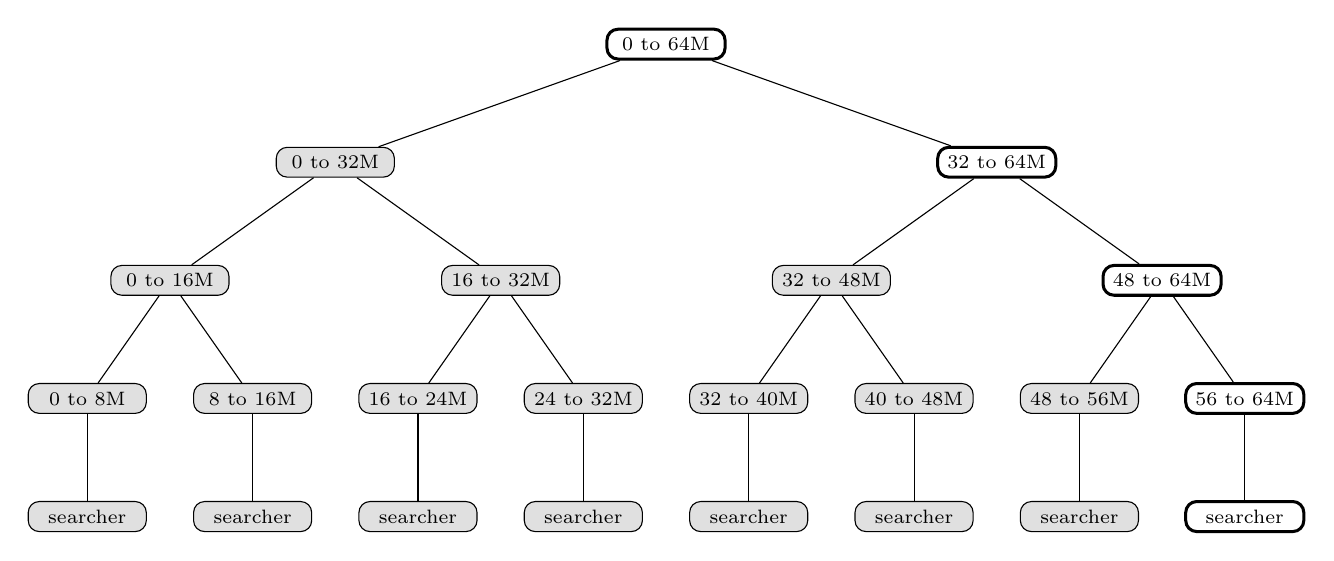
\begin{tikzpicture}[
	level distance=1.5cm,
	every node/.style={font=\scriptsize},
	part/.style={draw, rounded corners, inner sep=3pt, minimum width=1.5cm, align=center},
	killed/.style={draw, rounded corners, inner sep=3pt, minimum width=1.5cm, align=center, fill=black!12},
	win/.style={draw, rounded corners, inner sep=3pt, minimum width=1.5cm, align=center, line width=1.1pt},
	level 1/.style={sibling distance=8.4cm},
	level 2/.style={sibling distance=4.2cm},
	level 3/.style={sibling distance=2.1cm},
	level 4/.style={sibling distance=2.1cm}
]
\node[win] {0 to 64M}
	child {node[killed] {0 to 32M}
		child {node[killed] {0 to 16M}
			child {node[killed] {0 to 8M} child {node[killed] {searcher}}}
			child {node[killed] {8 to 16M} child {node[killed] {searcher}}}
		}
		child {node[killed] {16 to 32M}
			child {node[killed] {16 to 24M} child {node[killed] {searcher}}}
			child {node[killed] {24 to 32M} child {node[killed] {searcher}}}
		}
	}
	child {node[win] {32 to 64M}
		child {node[killed] {32 to 48M}
			child {node[killed] {32 to 40M} child {node[killed] {searcher}}}
			child {node[killed] {40 to 48M} child {node[killed] {searcher}}}
		}
		child {node[win] {48 to 64M}
			child {node[killed] {48 to 56M} child {node[killed] {searcher}}}
			child {node[win] {56 to 64M} child {node[win] {searcher}}}
		}
	};
\end{tikzpicture}
}
\caption{Part III. Thick outlines are the processes on the path from the successful
searcher to the root, which carry the exit status upward. Shaded nodes are the
three subtrees that receive \texttt{SIGTERM}, one per level.}
\label{fig:kill}
\end{figure}

\subsection*{What the log looks like in practice}
The number of \texttt{received SIGTERM} lines is not the same on every run. Over ten
consecutive runs on the same machine we saw anywhere between 0 and 13 of them. Two
effects explain the spread.

The first is that a process can only be killed if it is still alive. The file is 64
MiB and sits in the page cache after the first run, so a searcher often finishes its
8 MiB chunk before the good news has climbed three levels of the tree. On three of
the ten runs every single searcher had already finished and the whole run produced
no \texttt{SIGTERM} at all, which is a correct outcome and not a bug. It just means
the cancellation had nothing left to cancel.

The second is a genuine race between \texttt{fork} and \texttt{exec}. A searcher
installs its handler only after \texttt{execl} has replaced the process image, and
\texttt{exec} resets inherited handlers back to the default. If \texttt{SIGTERM}
lands inside that narrow window the process dies silently on the default action
instead of printing its message. The process is still terminated, so the behaviour
is correct, but its line is missing from the log. We saw this once during testing.

We also checked with \texttt{pgrep} after every run that no partitioner or searcher
was left behind, and none ever was.

\section*{Notes and Problems Encountered}

\begin{itemize}
	\item \textbf{Duplicated output.} The first version printed with
	\texttt{"{\textbackslash}n"}
	and no flush. On a terminal \texttt{cout} is line buffered so this looks fine,
	but as soon as the output was redirected to a file it became block buffered, and
	every \texttt{fork} handed a copy of the unflushed buffer to the child. Lines
	appeared twice. Flushing before each fork and after each message fixed it.
	\item \textbf{Chunk boundaries.} Chunks are disjoint and each searcher reads only
	its own range, so a pattern that straddles a boundary would be missed by both
	neighbours. The pattern here is 8 bytes and sits well inside chunk 8, so it does
	not bite, but a correct general solution would need each searcher to read a few
	extra bytes past its end.
	\item \textbf{Reusing \texttt{argv[0]}.} Passing \texttt{argv[0]} to
	\texttt{execl} instead of hard coding the binary name means the partitioner
	relaunches whatever binary was actually started. The searcher path is still hard
	coded because it is a different program.
	\item \textbf{Positions are \texttt{int}.} The largest position in this
	assignment is 67108863, which fits comfortably. A file above 2 GiB would need
	\texttt{long} and \texttt{seekg} with a wider offset type.
\end{itemize}

\section*{Building and Running}

\begin{verbatim}
make build-part1    make run-part1    clean-part1
make build-part2    make run-part2    clean-part2
make build-part3    make run-part3    clean-part3
make build-all      make clean
\end{verbatim}

The run targets use \texttt{file.txt}, the pattern \texttt{NGTNIJGK}, the range 0 to
67108863 and a maximum chunk size of 8388608.

\section*{Conclusion}
Part I gave a single process that scans a range and reports an absolute position.
Part II turned that into a tree of 23 processes built by repeated halving, where
creation flows down from the root and termination flows back up because every parent
is blocked in \texttt{wait}. Part III added a return path for the answer and a
signal path for the cancellation, and cut the work down to the branches that had not
already finished. The remaining rough edge is the fork to exec window in which a
searcher cannot yet report the signal that kills it.

\newpage
\section*{Appendix A: Full Output of Part II}
\begin{footnotesize}
\begin{verbatim}
[30824] start position = 0 ; end position = 67108863
[30824] forked left child 30825
[30824] forked right child 30826
[30825] start position = 0 ; end position = 33554431
[30826] start position = 33554432 ; end position = 67108863
[30825] forked left child 30827
[30826] forked left child 30828
[30825] forked right child 30829
[30826] forked right child 30830
[30827] start position = 0 ; end position = 16777215
[30828] start position = 33554432 ; end position = 50331647
[30829] start position = 16777216 ; end position = 33554431
[30827] forked left child 30831
[30828] forked left child 30832
[30829] forked left child 30833
[30830] start position = 50331648 ; end position = 67108863
[30827] forked right child 30834
[30828] forked right child 30835
[30829] forked right child 30836
[30830] forked left child 30837
[30830] forked right child 30838
[30832] start position = 33554432 ; end position = 41943039
[30833] start position = 16777216 ; end position = 25165823
[30834] start position = 8388608 ; end position = 16777215
[30831] start position = 0 ; end position = 8388607
[30835] start position = 41943040 ; end position = 50331647
[30832] forked searcher child 30839
[30836] start position = 25165824 ; end position = 33554431
[30833] forked searcher child 30840
[30837] start position = 50331648 ; end position = 58720255
[30834] forked searcher child 30841
[30835] forked searcher child 30843
[30831] forked searcher child 30842
[30838] start position = 58720256 ; end position = 67108863
[30837] forked searcher child 30845
[30838] forked searcher child 30846
[30836] forked searcher child 30844
[30846] found at 64520807
[30838] searcher child returned
[30830] right child returned
[30845] didn't find
[30841] didn't find
[30844] didn't find
[30837] searcher child returned
[30840] didn't find
[30843] didn't find
[30839] didn't find
[30834] searcher child returned
[30842] didn't find
[30836] searcher child returned
[30832] searcher child returned
[30830] left child returned
[30833] searcher child returned
[30835] searcher child returned
[30831] searcher child returned
[30828] left child returned
[30829] right child returned
[30826] right child returned
[30827] right child returned
[30829] left child returned
[30827] left child returned
[30828] right child returned
[30825] right child returned
[30825] left child returned
[30826] left child returned
[30824] left child returned
[30824] right child returned
\end{verbatim}
\end{footnotesize}

\newpage
\section*{Appendix B: Full Output of Part III}
\begin{footnotesize}
\begin{verbatim}
[31116] start position = 0 ; end position = 67108863
[31116] forked left child 31117
[31116] forked right child 31118
[31117] start position = 0 ; end position = 33554431
[31117] forked left child 31119
[31117] forked right child 31120
[31118] start position = 33554432 ; end position = 67108863
[31118] forked left child 31121
[31118] forked right child 31122
[31119] start position = 0 ; end position = 16777215
[31119] forked left child 31123
[31120] start position = 16777216 ; end position = 33554431
[31119] forked right child 31124
[31120] forked left child 31125
[31121] start position = 33554432 ; end position = 50331647
[31122] start position = 50331648 ; end position = 67108863
[31121] forked left child 31127
[31122] forked left child 31128
[31122] forked right child 31130
[31123] start position = 0 ; end position = 8388607
[31124] start position = 8388608 ; end position = 16777215
[31123] forked searcher child 31131
[31124] forked searcher child 31132
[31125] start position = 16777216 ; end position = 25165823
[31128] start position = 50331648 ; end position = 58720255
[31127] start position = 33554432 ; end position = 41943039
[31128] forked searcher child 31134
[31127] forked searcher child 31135
[31121] forked right child 31129
[31126] start position = 25165824 ; end position = 33554431
[31129] start position = 41943040 ; end position = 50331647
[31120] forked right child 31126
[31125] forked searcher child 31133
[31129] forked searcher child 31137
[31126] forked searcher child 31136
[31130] start position = 58720256 ; end position = 67108863
[31130] forked searcher child 31138
[31131] didn't find
[31135] didn't find
[31123] searcher child returned
[31127] searcher child returned
[31119] left child returned
[31121] left child returned
[31132] didn't find
[31138] found at 64520807
[31124] searcher child returned
[31130] searcher child returned
[31119] right child returned
[31122] right child returned
[31117] left child returned
[31128] received SIGTERM
[31118] right child returned
[31121] received SIGTERM
[31129] received SIGTERM
[31116] right child returned
[31117] received SIGTERM
[31120] received SIGTERM
[31126] received SIGTERM
[31125] received SIGTERM
[31136] received SIGTERM
[31134] received SIGTERM
[31133] received SIGTERM
[31137] received SIGTERM
\end{verbatim}
\end{footnotesize}

\end{document}
